\documentclass[a4paper,11pt]{article}
\usepackage[utf8]{inputenc}
\usepackage{titling}
\usepackage[a4paper,margin=0.75in]{geometry} % Adjust the margins here
\usepackage{amsmath,amssymb,amsfonts}
\usepackage{algorithmic}
\usepackage{graphicx}
\usepackage{textcomp}
\usepackage{comment}
\usepackage{xcolor}
\usepackage{enumitem}
\usepackage{tcolorbox}
\usepackage{listings}
\tcbuselibrary{listings,skins}  

\usepackage{changepage}

\usepackage{caption}
\usepackage{draftwatermark}
\usepackage{environ}

\usepackage{lmodern} % Optional: Use a scalable font family
\usepackage{scalefnt} % Optional: Allow smooth font scaling

\usepackage{siunitx} % ohm symbol

\usepackage{fancyvrb}     % for the Verbatim environment
% Customize watermark
\SetWatermarkText{\scalefont{1.5}GOWDA} % Use scalefont for scaling
\SetWatermarkScale{.2} % Adjust scale to avoid very large fonts
\SetWatermarkColor[gray]{0.7} % Light gray (80% white)
\SetWatermarkAngle{30}
%\SetWatermarkHorCenter{8cm} % Move right by 3 cm
%\SetWatermarkVerCenter{18cm} % Move up by 12 cm




\newtcblisting{codebox}[2][]{%
  colback=blue!10,           
  colframe=black,                       
  boxrule=1pt,               
  title={#2},                
  listing only,              
  listing engine=listings,   
  listing options={%
    language=Python,
    upquote = true,
    basicstyle=\ttfamily\small,
    breaklines=true,
    showstringspaces=false,
    frame=none,
    xleftmargin=0pt,
    xrightmargin=0pt,
    aboveskip=0pt,
    belowskip=0pt,
    #1
  },
}

\newtcblisting{outputs}[1][]{%
  colback=green!10,
  colframe=black,
  boxrule=1pt,
  title={Output:},
  listing only,
  listing engine=listings,
  listing options={%
    language=Python,
    upquote = true,
    basicstyle=\ttfamily\small,
    commentstyle=\ttfamily\small,
    breaklines=true,
    showstringspaces=false,
    frame=none,
    xleftmargin=0pt, xrightmargin=0pt, aboveskip=0pt, belowskip=0pt,
    columns=fullflexible,
    #1
  },
}

\newtcblisting{syntax}[1][]{%  ← only one optional argument now
  colback=red!10,
  colframe=black,
  boxrule=1pt,
  title={Syntax:},         % ← fixed, constant title
  listing only,
  listing engine=listings,
  listing options={%
    language=Python,
    upquote=true,
    basicstyle=\ttfamily\small,
    breaklines=true,
    showstringspaces=false,
    frame=none,
    xleftmargin=0pt,
    xrightmargin=0pt,
    aboveskip=0pt,
    belowskip=0pt,
    #1                            % any per-box overrides
  },
}


\title{Introduction to Programming \\ Lab: Understanding Functions}
\author{Vikas Thammanna Gowda}
\date{07/29/2025}

\lstset{
    language=Python,
    basicstyle=\ttfamily\small,
    keywordstyle=\bfseries,
    showstringspaces=false,
    breaklines=true,
    frame=none,
    xleftmargin=5pt,
    xrightmargin=5pt,
    aboveskip=10pt,
    belowskip=5pt,
    captionpos=b
}
\begin{document}
\maketitle

\noindent \textbf{Name: \_\_\_\_\_\_\_\_\_\_\_\_\_\_\_\_\_\_\_\_\_\_\_\_\_\_\_\_\_\_\_\_\_\_\_\_\_\_\_\_\_\_\_\_\_\_\_}
\section*{Introduction}
In this lab, you will build and program a Raspberry Pi circuit to play a Rock-Paper-Scissors game against the computer using three buttons, LEDs, and a character LCD.

\begin{itemize}
\item \textbf{Part 1:} You will be provided with the \textit{complete code, circuit diagram, setup, 
and wiring instructions}, along with a \textit{brief in-class demonstration}. 
You will press a button to make a move; the LCD will display your choice, the computer's choice, and the result.

\item \textbf{Part 2:}  Enhance the code by refactoring repeated logic into functions 
and adding multiple game modes (Sudden Death, Best of 3, First to 3 Wins). 
This activity illustrates how user-defined functions promote reuse and clarity.
\end{itemize} 

\subsection*{Learning Objectives}
\begin{itemize}
    \item Understand definition and invocation of Python functions.

\item Apply functions to encapsulate game logic and avoid repetition.

\item Observe how loop structure controls the timing and order of physical outputs.

\item Integrate user input (buttons) and output (LCD, LEDs) in an event-driven program

\item Design program flow for different game‑mode rules.

\item Learn to use the \texttt{finally} block to ensure cleanup actions (like turning off LEDs) are always executed.
\end{itemize}

\subsection*{Required Components:}
\begin{itemize}
    \item Raspberry Pi (any model with 40 GPIO pins) with Raspbian/Raspberry Pi OS installed. 
\item Breadboard and jumper wires.
\item 3 bottons, LCD display for Part 1. 
\item For Part 2, you will choose the componenets to enhance your project, LEDs, resistors, and additional buttons as needed.

\end{itemize}


\newpage
\section*{Part 1: Single Round RPS}
In Part 1, students use three GPIO-connected push-buttons and a 20$\times$4 character 
LCD to implement a single-round Rock-Paper-Scissors game entirely in software. 
As soon as the script starts, it blocks waiting for one of the buttons to be pressed—each button representing rock, 
paper, or scissors—and then immediately sends that choice to the LCD. 
The program simultaneously generates a random “computer” choice, and 
the LCD briefly displays both selections 
(for example, “You: Paper” on the top line and “CPU: Scissors” on the bottom line). 
After a one-second pause, the script computes the outcome using a simple modulo-3 
check and replaces the display with “You Win,” “You Lose,” or “Draw” for 
two seconds before clearing the screen and returning to wait for the next button press. 
This exercise gives students hands-on practice with reading button input, writing text to an LCD, 
blocking for user input, and implementing core game-logic in Python.


\subsection*{Illustration}

Follow these steps to assemble the circuit.
These instructions describe how to wire three tactile push-buttons to a Raspberry Pi using its GPIO pins and the breadboard's 
ground rail. Each button will serve as an input for the Rock-Paper-Scissors game: 
Button 1 for Rock, Button 2 for Paper, and Button 3 for Scissors. 
Internal pull-up resistors on the Pi will hold each input high until the button is pressed, pulling it to ground.
\textbf{Make sure your Raspberry Pi 
is shut down or powered off while wiring the circuit to avoid any accidental 
short circuits or damage.}

    \begin{figure}[h] % 'h' places the figure approximately here
        \centering
        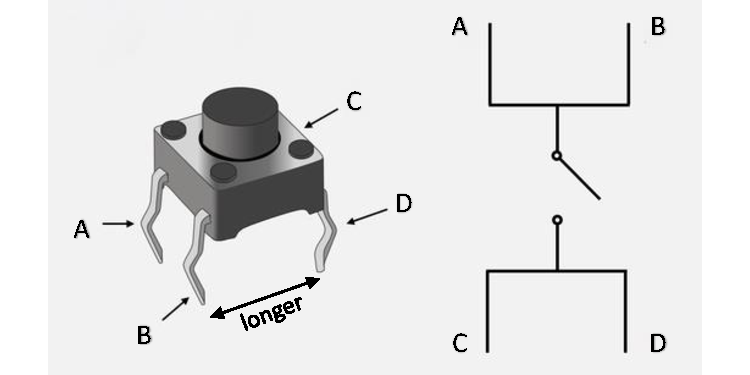
\includegraphics[width=1\textwidth]{fig4.pdf} % Change size as needed
        \caption{Button internal circuit.}
        \label{fig:button1}
    \end{figure}

\subsubsection*{Button Wiring}
\begin{enumerate}
    \item \textbf{Prepare the Breadboard:} Before wiring any components, establish a common ground reference between 
    the Raspberry Pi and the breadboard. This ensures that when a button is pressed, the Pi correctly detects a LOW signal. 
    Connect a jumper from the Raspberry Pi's GND pin to the breadboard's ground (-) rail.
\newpage
    \item \textbf{Place the Tactile Switches:} Tactile switches have four legs arranged in two electrically connected pairs. 
    Mounting them across the central trench ensures that pressing the switch closes the circuit between those pairs.  
    Orient each switch so that its two pairs of legs straddle the central trench of the breadboard.
    Verify that pressing the button connects the two legs on one side to the two legs on the opposite side.

    
    \begin{figure}[h] % 'h' places the figure approximately here
        \centering
        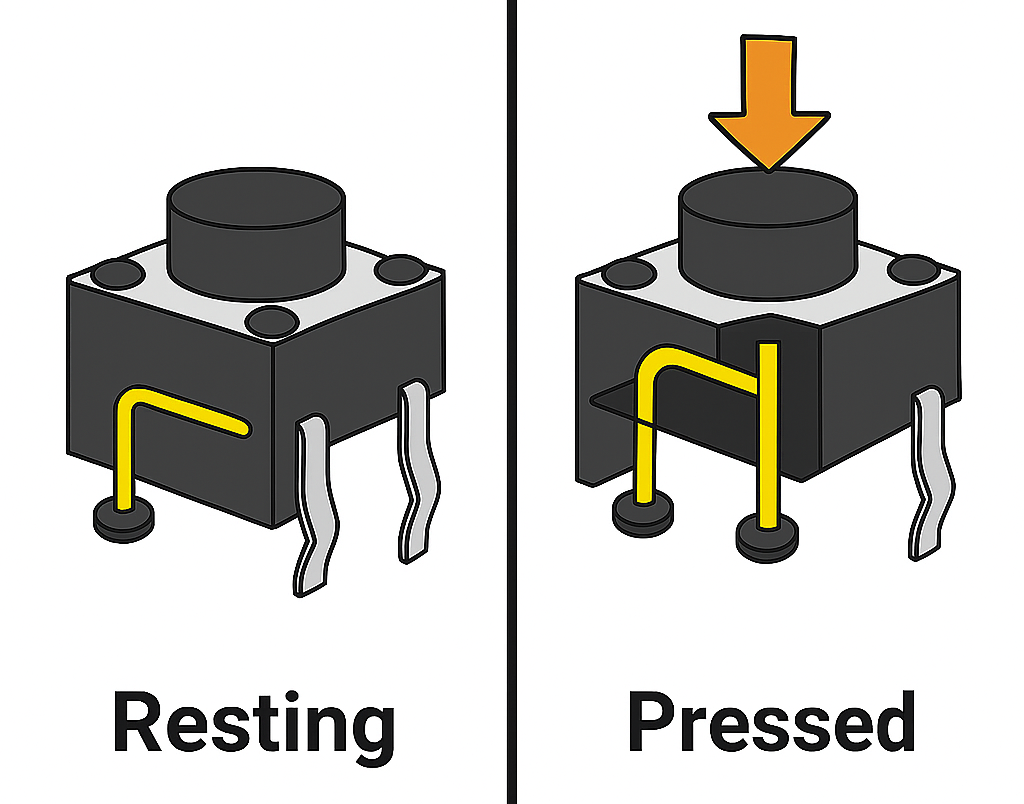
\includegraphics[width=.5\textwidth]{fig3.png} % Change size as needed
        \caption{Circuit Diagram.}
        \label{fig:button}
    \end{figure}

    \item \textbf{Wire the Buttons:} Each button input uses one GPIO line and the ground rail. 
    When the button is not pressed, the internal pull-up holds the GPIO pin at a logical HIGH. 
    Pressing the button connects it to ground, producing a logical LOW that the program can detect.
    \begin{itemize}
        \item Connect one leg of each button to the ground rail (-) on the breadboard.
        \item Connect the other leg of Button 1 to GPIO 26 (physical pin 37 on the Pi).
        \item Connect the other leg of Button 2 to GPIO 20 (physical pin 38).
        \item Connect the other leg of Button 3 to GPIO 21 (physical pin 40).
    \end{itemize}
    \begin{figure}[h] % 'h' places the figure approximately here
        \centering
        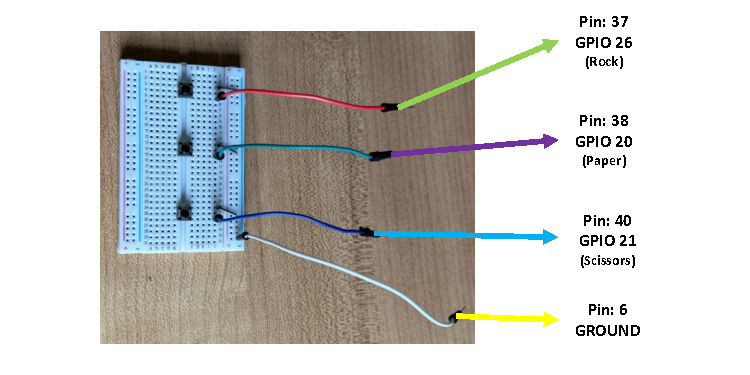
\includegraphics[width=1\textwidth]{fig1.pdf} % Change size as needed
        \caption{Buttons set-up.}
        \label{fig:runtime}
    \end{figure}

\end{enumerate}


\subsubsection*{LCD Display Wiring:}
For the 20$\times$4 character LCD, we assume it has an I²C interface adapter attached. 
This adapter greatly simplifies the wiring by using only four connections.

\begin{figure}[h] % 'h' places the figure approximately here
    \centering
    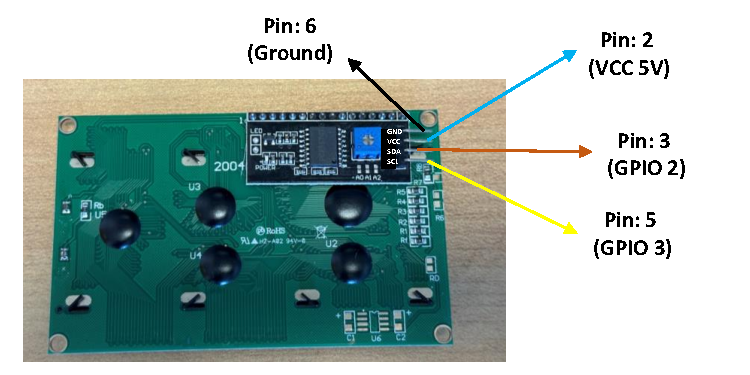
\includegraphics[width=.85\textwidth]{fig5.pdf} % Change size as needed
    \caption{LCD connection to Raspberry Pi's GPIO pins.}
    \label{fig:LCD}
\end{figure}

\begin{enumerate}
    \item Connect the LCD module's VCC pin to the Pi's 5V power (physical pin 2 or 4), 
    and the LCD GND to a Pi GND pin 6.

    \item Connect the LCD’s SDA pin to the Pi’s SDA line. On Raspberry Pi, SDA corresponds to GPIO 2 (physical pin 3)

    \item Connect the LCD's SCL pin to the Pi's SCL line, which is GPIO 3 (physical pin 5).

\end{enumerate}


\subsection*{Complete Setup}
\begin{figure}[h] % 'h' places the figure approximately here
    \centering
    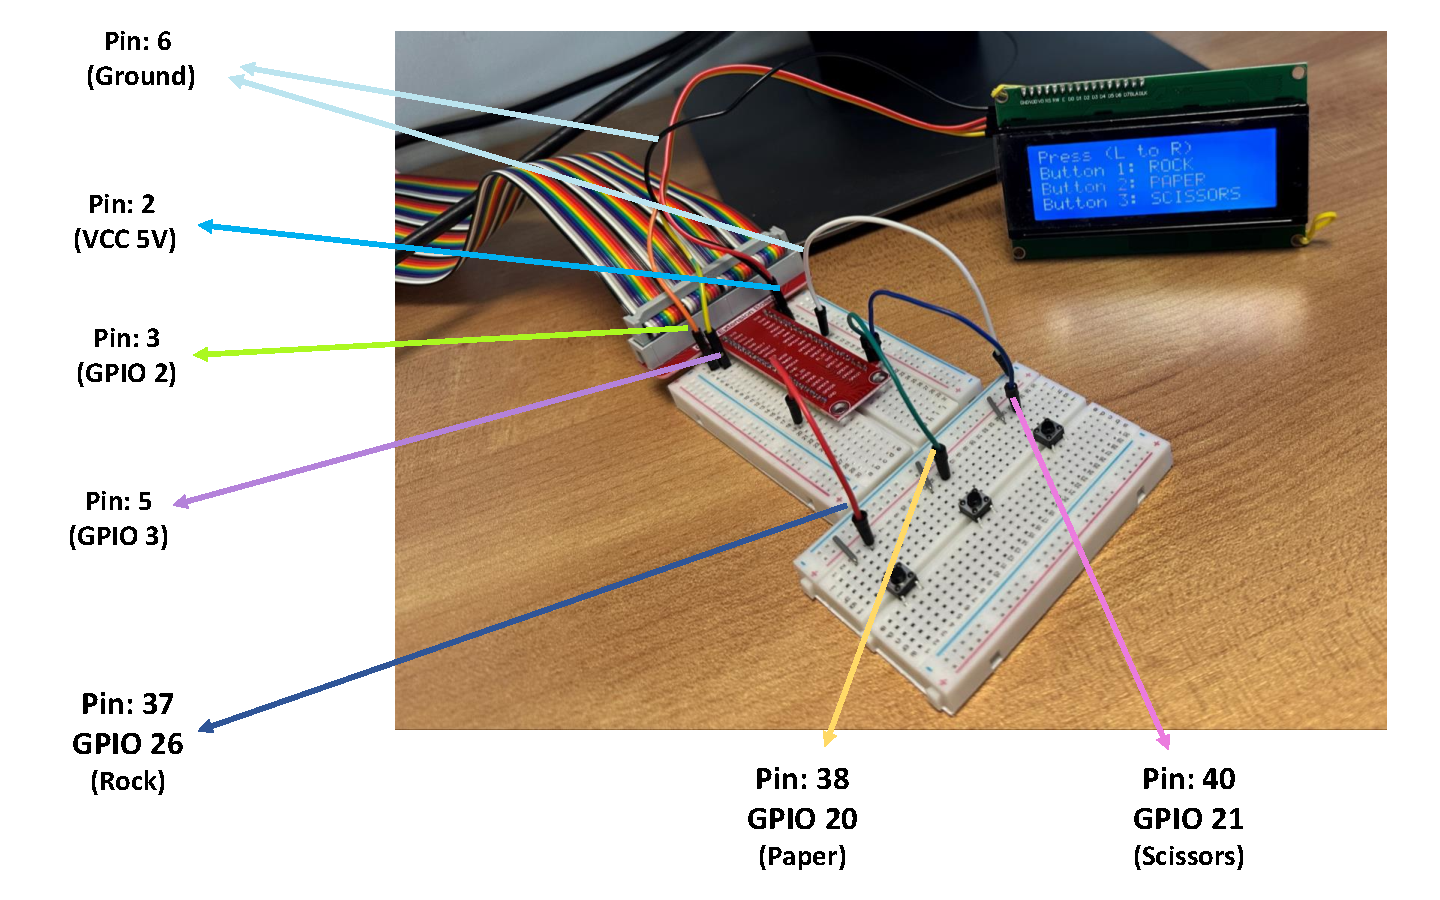
\includegraphics[width=.85\textwidth]{fig2.pdf} % Change size as needed
    \caption{Wiring set-up.}
    \label{fig:runtime1}
\end{figure}
\newpage
\subsection*{Run and Observe}
It’s time to test the circuit and code. Make sure your 
Raspberry Pi is powered on and the circuit is connected as described. 
Run the privided code.

\subsection*{Record your observations:}
\begin{table}[ht]
  \centering
  \renewcommand{\arraystretch}{1.5}
  \begin{tabular}{|p{4cm}|p{4cm}|p{4cm}|}
    \hline
    \textbf{Computer Choice} & \textbf{User Choice} & \textbf{Result} \\ \hline
     &  &  \\ \hline
     &  &  \\ \hline
     &  &  \\ \hline
     &  &  \\ \hline
     &  &  \\ \hline
     &  &  \\ \hline
     &  &  \\ \hline
     &  &  \\ \hline
  \end{tabular}
  \caption{Gane Results}
  \label{tab:empty-3x10}
\end{table}


\newpage
\section*{Part 2: Enhanced Game Modes }
In Part 2, students take the working single‐round game from Part 1 and transform it into a clean, 
modular program by creating user‐defined functions for each core task—such as reading a button press, 
displaying messages on the LCD, and determining the winner of a round. They then build three distinct 
game‐mode loops (Sudden Death, Best of 3, and First to 3 Wins) that simply call these functions instead of 
retyping the same code, reinforcing how functions promote clarity, reduce duplication, and make complex programs 
easier to extend and maintain.

\subsection*{Tips for Implementation}
\begin{itemize}
  \item \textbf{Modularizing the core logic:} Students begin by defining focused functions—such as \\ \texttt{get\_choice()}, \texttt{display\_message()}, and \texttt{decide\_winner()}—each responsible for a single task. This separation makes the code more readable and easier to test or modify.
  \item \textbf{Eliminating repetition:} By invoking these functions wherever the associated behavior is needed, rather than copying-and-pasting code, students learn the DRY principle (Don't Repeat Yourself) and experience firsthand how refactoring reduces bugs and duplication.
  \item \textbf{Adding a mode-selection menu:} Before the game loop starts, the program displays an LCD menu letting the user choose between Sudden Death, Best of 3, or First to 3 Wins. This step introduces branch logic and menu navigation on the LCD.
  \item \textbf{Implementing Sudden Death mode:} In this simplest mode, the code calls a \texttt{play\_round()} function exactly once and then immediately shows the winner. It illustrates how a single function call can encapsulate an entire round.
  \item \textbf{Implementing Best of 3 mode:} Students write a loop that repeatedly calls \texttt{play\_round()} until either the user or the CPU wins two rounds, reinforcing loop constructs, condition checks, and state tracking of win counts.
  \item \textbf{Implementing First to 3 Wins mode:} This mode extends the loop logic to continue playing until a player reaches three wins, teaching students how to manage cumulative state and termination conditions over an indefinite number of rounds.
  \item \textbf{Incorporating LED enhancements:}
    \begin{itemize}
      \item Encourage students to use the existing GPIO-connected LEDs as visual feedback—e.g., blink all three rapidly during mode selection, then light only the chosen mode’s LED.
      \item Define a helper function like \texttt{blink\_led(led, times)} to signal round start/end or to indicate a win (three quick blinks) versus a loss (single long blink).
      \item Use slow/fast blink patterns on the runner LEDs to reinforce the slowing animation in each game mode.
    \end{itemize}
  \item \textbf{Displaying final results:} After the chosen mode completes, the program uses \\ \texttt{display\_message()} to show the final score tally and announce the overall winner on the LCD, demonstrating composition of functions for user feedback.
\end{itemize}




\newpage
\section*{Reflection and Analysis}
\begin{enumerate}
    \item Why use functions? Explain how they improve readability and reduce duplication.

    \item Mode logic: For each mode, outline in pseudocode how you check win counts.

    \item LCD feedback: How does encapsulating display calls in a function simplify changes (e.g., adding animations)?

    \item \textbf{Further extension:} Discuss how this project can be extended. 

\end{enumerate}

\end{document}